\documentclass[main.tex]{subfiles}
\begin{document}

\chapter{Research}

As with any project, it is vital to be informed about existing solutions and technology within the given field of computing. As such, we conducted a wide array of research relating to smartphones and existing indoor navigation technology.

%In this section, we will be presenting the research carried out over the course of the project. We will be looking into the technology available within modern smartphones and also the tools that are provided to create applications for these phones. We shall also be analysing various solutions that have been developed within the field of indoor navigation.

 \section{Tracking user movement}

An obvious way to track user position is to perform double integration on the obtained acceleration to get distance travelled. However this results in introduction of error, as the result is only an approximation of the underlying signal. Furthermore, integration of the noise component leads to the standard deviation of the error in position increasing with integration time~\cite[p.73]{integrationError}. Thong, Y. K., et al.~\cite{integrationErrorPractical} analysed the practical effect that double integration of accelerometer noise has on this error by carrying out experiments using two commercial accelerometers, and found that this error very quickly accumulates with time~\cite[p.1168]{integrationErrorPractical}. As such, this approach is deemed unsuitable for a navigation system which continuously and precisely requires the user’s current position. Foxlin, E.'s approach~\cite{foxlin2005pedestrian} alleviates the integration error by using the concept of `zero-velocity updates (ZUPTs)’, which exploits the fact that there is a momentary stationary period of zero velocity and acceleration during walking motion when the user’s foot makes contact with the ground. This allows correction of the velocity error after each stride and makes the error accumulation ``linear in the number of steps''~\cite[p.38]{foxlin2005pedestrian}. This, however, requires a dedicated sensor to be placed on the user’s foot and does not come under the purview of a smartphone based approach. 

Most dead-reckoning systems thus make use of step detection to identify user movement and step length estimation to estimate their displacement and avoid the double integration problem. Existing approaches that make use of a smartphone’s inertial sensors typically restrict the phone’s position to two scenarios - the user having the phone in their pocket and/or in front of them in their hand. Steps are detected by identifying the consistent change in sensor readings, particularly the accelerometer, caused by rythmic motion during walking. For instance, Wang, H., et al.~\cite{wang2012no} observe that the graph of magnitude readings of a 3-axis accelerometer follow a sinusoidal pattern corresponding to the ``natural up/down bounce of the human body for each step taken''~\cite[p.203]{wang2012no} in both the in-hand and pocket case. They then isolate individual steps through simple peak detection and thresholding in the graph. Li, F., et al.~\cite{li2012reliable} also use accelerometer magnitude in a similar manner to identify steps, subsequently applying heuristic constraints and dynamic time warping validation to reduce false positives.  

While taking the magnitude of the accelerometer allows the step detection procedure to be independent of the phone’s orientation, as a side effect, moving the phone along the axes that do not correspond to the user’s vertical movement can also produce similar sinusoidal patterns. Jin, Y., et al.~\cite{jin2011robust} isolate acceleration specifically along the required vertical axis by projecting the acceleration measurements from the phone’s local x-y-z axes to the East-North-Up (E-N-U) world co-ordinate system, where `Up' is the desired axis.  This is achieved by using the `rotation matrix' containing orientation measurements that are applied to the acceleration vector in the local co-ordinates. Once the accelerometer readings are obtained on this vertical axis they detect steps by identifying sequences of local maximas followed by local minimas along with thresholding on both the time elapsed and absolute value difference between the two. 

Efforts have also been made to extend step detection to work in arbitrary phone positions, so that it can be used in real-world situations where the position varies as the user performs a multitude of activities. Such approaches either involve broadly identifying the type of activity the user is performing and then using the appropriate sensors for step detection in that particular situation, or generating and using one or more measures that already take into account the variations in position. Susi, M., et al.~\cite{susi2013motion} specify a set of possible user activities and associate with each one unique features based on measures derived from accelerometer and gyroscope readings. The user’s current activity is then identified by extracting the feature set corresponding to their motion and using a pre-defined decision tree to classify it as one of the specified activities. A specific version of the algorithm optimised for peak detection in the context of that particular activity is then used to detect steps. For instance, if the activity is classified as `phone in swinging hand' then gyroscope readings are also considered due to periodic rotation of the user’s arm. Conversely, activities such as texting do not involve any rotation and thus only accelerometer readings are looked at. Zeng, Q., et al.~\cite{zeng2015novel} proposed a novel step counting algorithm that works irrespective of the phone’s position and step mode (variation in the user’s motion, including walking and running). In addition to the accelerometer they also make use of the 3-axis gravity sensor, which provides acceleration acting on each of the axes specifically due to gravity. A change in these values signifies a change in the position/orientation of the phone and can be used to compensate for the resulting variance in accelerometer readings. Thus the authors take a linear combination of the accelerometer and gravity readings to produce a single metric incorporating this compensation, on the basis of which step detection is carried out. Lee, H., et al.~\cite{lee2015step} consider both the short and long term changes in accelerometer magnitude to capture the variations caused due to different positions and step modes. Peak/valley candidates are identified on the basis of measures that track these short/long term changes such as mean and standard deviation. Candidates are then validated using adaptive thresholds which ensure that sufficient time, corresponding to the estimated minimum duration between subsequent steps in standard motion, has elapsed between adjacent peaks and valleys. 

\subsection{Step Detection}

Step detection is one of the most vital components of the navigation system as it is the basis on which a user's motion is detected. In a dead-reckoning system a user's current position is determined by incrementally estimating their displacement from a previously known position. Thus if the user's starting location is known, step detection along with the user's bearing can be used to identify when they have moved and along which direction. Combining this with step length estimation allows for determining the magnitude of this displacement, which enables keeping track of the user's position as they navigate within the mapped area. 

Algorithms for step detection using smartphones typically analyse the phone's sensor readings and relate them to the user's movement. Deciding on which specific sensors to analyse and the algorithms to apply on them is dependent on the exact placement of the phone while the user walks. The two situations commonly considered are the `in-pocket' case, where the phone is kept in the user's pant pocket near hip level and the `in-hand' case, where the user keeps the phone in their hand and directly in front of them at around chest level. 

\section{Sensors Considered}

\subsection{Accelerometer}
Existing approaches predominantly make use of the phone's accelerometer readings in order to detect the user's steps. As the name suggests, an accelerometer is a device that measures the acceleration that is applied to the device. In smartphones, this acceleration $A_{d}$ is measured using the relation in 
Equation~\ref{eq:accelerometerAcceleration}~\cite{accelerometerAcceleration}.  

\begin{equation}\label{eq:accelerometerAcceleration}
A_{d} = - \sum F_{s}/massAccelerometer
\end{equation}
\\
where $\sum F_{s}$ is the sum of the forces acting upon the device. Included in $F_{s}$ is the force acting on the device due to the Earth's gravity, which produces acceleration having a constant magnitude of $9.81 m/s^2$. 

In particular, most modern smartphones come equipped with a `3-axis' accelerometer, which reports the accelerations acting separately on the 3 principal axes of the phone's co-ordinate system - X, Y and Z. In Android and iOS these 3 axes are defined relative to the phone's screen when held in its `natural orientation', which is portrait in most cases. The axes are illustrated in Figure~\ref{fig:axisDevice}

\begin{center}
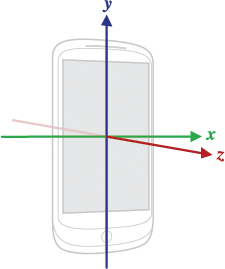
\includegraphics[scale=0.5]{images/axisDevice.png}
\captionof{figure}{The 3 principal axes of smartphones, defined with respect to the screen in its `natural orientation'~\cite{axisDevice}}
\label{fig:axisDevice}
\end{center}

As seen from the figure, the X-axis passes through the side of the phone, the Y-axis is along the vertical segment while the Z-axis projects out from the center of the screen. The positions of these axes remain fixed with respect to the screen, and thus rotate accordingly along with change in the phone's orientation. 

In order to confirm that the actual sensor readings correspond to the described behaviour we recorded and analysed accelerometer data from our own phones. The first recording was performed with the phone remaining stationary throughout and kept flat on the surface with the screen facing upwards. The readings obtained are shown in Figure~\ref{fig:accelerationZ}.

\begin{center}
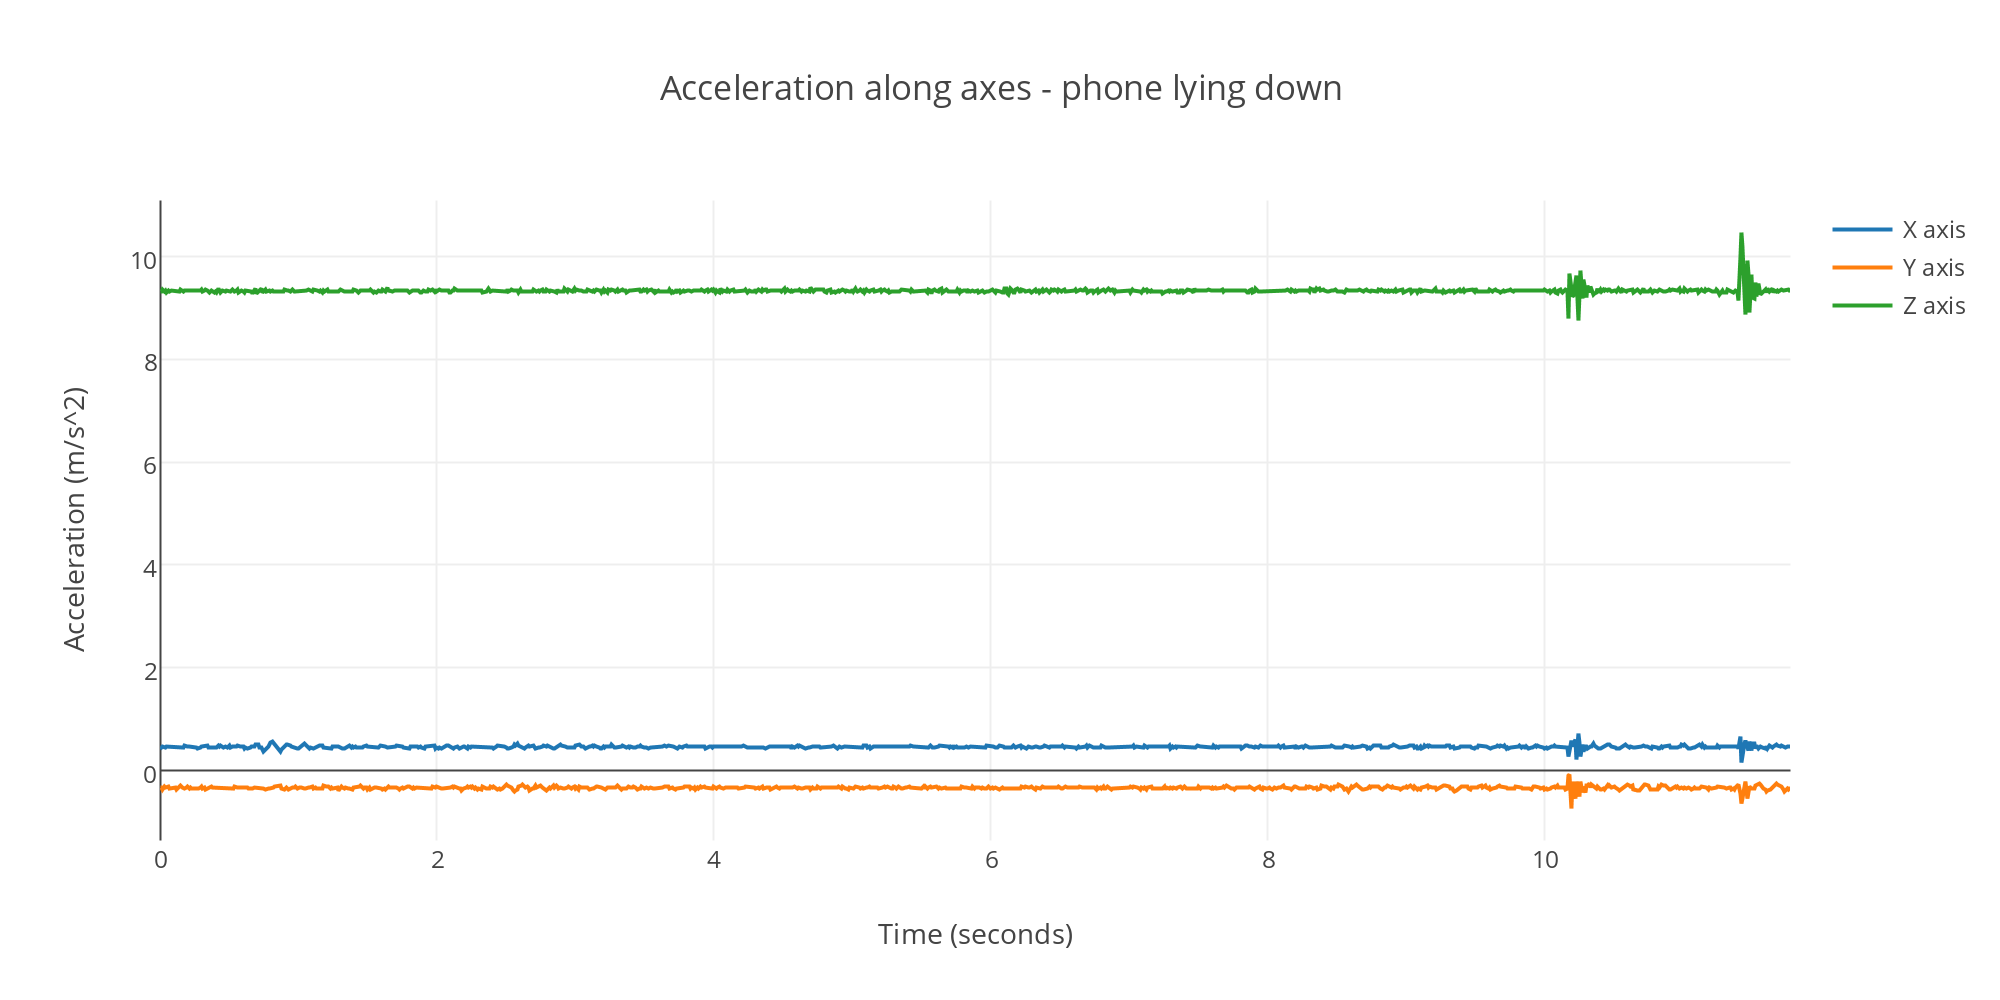
\includegraphics[scale=0.9]{images/accelerationZ.png}
\captionof{figure}{Accelerometer readings with phone kept flat on the surface}
\label{fig:accelerationZ}
\end{center}

As expected, the acceleration along the X and Y axes are close to 0, while there is a constant acceleration of about $9.81 m/s^2$ along the Z axis due to the force of gravity acting downwards through the screen of the phone. Note that the direction of acceleration in this case is upwards as the phone at rest accelerates upwards with respect to the local reference frame of a freely falling object close to the surface. 

This process is repeated with the phone held upright this time (with the bottom of the phone in contact with the surface). The obtained readings are shown in Figure~\ref{fig:accelerationY}.

\begin{center}
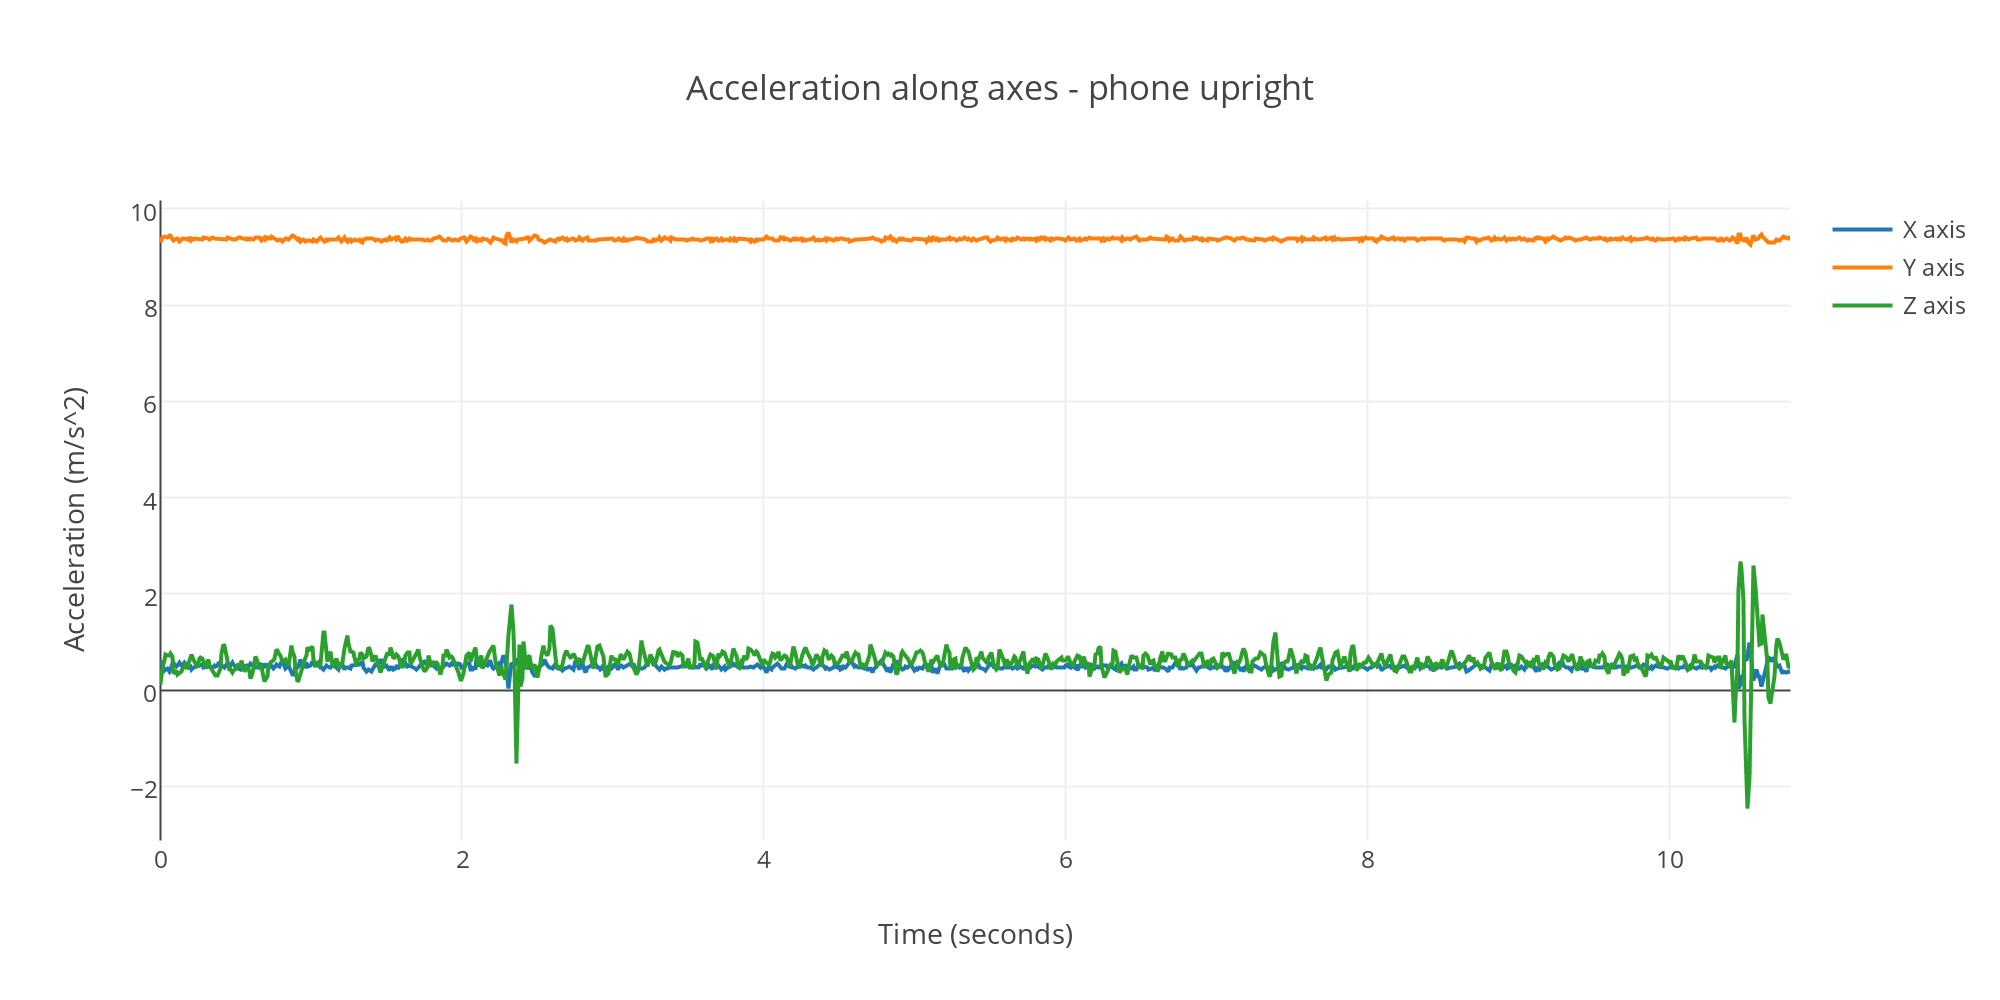
\includegraphics[scale=0.9]{images/accelerationY.png}
\captionof{figure}{Accelerometer readings with phone kept upright}
\label{fig:accelerationY}
\end{center}

The acceleration due to gravity is now along the Y-axis in accordance with the described behaviour, with the momentary spike in the Z-axis acceleration towards the end occurring due to slight movement of the hand while keeping the phone upright. On this basis it can also be concluded that keeping the phone lying on its side would make the gravity acceleration act along the X-axis, showing that the readings are consistent with the manner in which the phone's principal axes are defined. 
\\
\\
\subsection{Gyroscope}
In addition to the accelerometer some approaches also consider the readings from the gyroscope, which is a sensor that measures the rate of rotation around the phone's principal axes~\cite{accelerometerAcceleration}. Such rotations can be correlated with the user's steps in certain situations, such as when the phone swings while the user has their hand to the side of their body while walking. Since we envisaged any final application to have the phone's position be in the user's hand and in front of them at all times, there would be no considerable rotational motion involved. Thus the gyroscope readings will not provide any meaningful information for step detection and they are not considered in our approach. 

\subsection{Barometer}

As smartphones continue to get more and more powerful, new sensors are added to the array they already have. In recent years the barometer is becoming more prevelant. This a sensor that can determine the air pressure surrounding the phone. With this information, it is possible to obtain a height above sea level for the phone based of the barometric formula, which models the relationship from pressure to altitude.

The application of this information has the potential to be very useful and influential for indoor navigation systems, as if accurate enough, a barometer would allow for more precise vertical positioning, allowing systems to keep track of users throughout several floors in large buildings. With this in mind, a team from Singapore Management University ~\cite{baro2014} set out to test if barometric sensors in phones could be used for this purpose.

In their study they tested numerous factors that could have an effect on the readings, finding that  time, weather and location had an effect on the pressure values the sensors recorded. Although this was expected, the team was caught by surprise by the fact that even identical devices left next to one another would produce different pressure readings but with the same overall pattern. ~\cite[p.2]{baro2014}
%These three factors are expected to have an effect as it is well documented that weather has an effect on the pressure, and obviously with time and location the weather and conditions are likely to be given. The other unexpected factor that was found 

This lead them to instead of focusing on the absolute barometer reading, look at the relative reading, so the differences between changes in readings. This pressure difference is independent of all the above factors and therefore could be used to predict floor changes. After proving this was indeed the case, they moved on recording a number of samples and using data analysis techniques to see if they could predict whether a floor had changed just using the difference in pressure values. With this they managed to achieve a 99.54\% accuracy.

This particular study proves the potential that the barometer has in terms of indoor naviagtion and keeping track of a user's verticality. However it is noted that floors need to have a minimum difference of 0.2hPa or 1.6 metres, as the maximum error in pressure differences was around this value. If in a building the difference between floors is close to this value the probability of error increases.

Whilst this study proves that the barometer is useful, it isn't the only system that shows the uses of the barometer. Another example of this is the iBaro-altimeter system developed at The University of Tokyo ~\cite{baro22014}. To calculate ones altitude you need another reference point of pressure as part of the barometric formula, often either obtained from a nearby local source (meteorological station) or a through using a constant.

This system they proposed worked by using a series of standard reference points and other temporary ones they could ascertain to be correct, such as a smartphone in the system that they have assigned an altitude to. These collected reference points are stored on a server, then a smartphone that wants its altitude makes a request with some required information.

Whilst this system achieved low error rates, it requires a large amount of infrastructure which doesn't fit with the idea behind the applicaton. Even if the server could be removed from the design, an internet connection would be required to collect some of the reference points and GPS location is one of the inputs that the server wants to return an altitude.

\section{Landmarks}

Landmarks have long since been tools used for navigation, prior to the creation of smartphones and other technologies. It should then be of no surprise that some navigation methods for smarthphones have adopted these as the core of how they operate. For the purposes of this project, two different classes of landmark based systems were examined:

\begin{enumerate}
	\item \textbf{Beacon/Non-Organic Landmarks} - This is were wireless beacons are placed in the environment and the device uses them to determine it's location
	\item \textbf{Organic Landmarks} - This a system that uses landmarks that have been identified to be with in the environment, such as Wi-fi routers, elevators etc...
\end{enumerate}

Note the term Organic is a reference to the landmark being present in the environment without the need for the development team to place an object or device to create the waypoint.

An example of a Beacon based system is one developed by Inoue. Y, et. al ~\cite{Inoue2009} which works autonomously, removing the need for additional infrastructre in the form of a server. The beacons in this project are self-sufficient devices with their own power sources and transmitters, meaning that the required infrastructure is low-cost and able to placed in any location.

Prior to using the devices for , three sets of reference data are required:

\begin{enumerate}
	\item \textbf{Pedestrian Network Data} - Data that defines where a pedestrain can walk within the specified environment.
	\item \textbf{Bulding Map Data} - The floorplan for the building
	\item \textbf{Received Signal Strength (RSS) Fingerprint Data} - This is data that helps with locational calculations
\end{enumerate}

The RSS Fingerprint Data is obtained by measuring the RSS at fixed points in the environment for every beacon. From the reference data and real-time beacon signal data it is then possible to calculate where the user should be located. This application uses a series of particle filters to then estimate a position and keep updating it as new beacon data is recieved.

Whilst this approach reduces the amount of infrastructure normally required for beacon based approaches by not requiring a server, it still requires the placement of devices in the environment. This combined with the focus not being on the use of inertial sensors for navigation make it unviable for the scope of our requirements.

With Organic Landmarks the issue of not fitting the requirements of using inertial sensors is removed. Since there are longer devices placed in the environment to help with locational calculations. There are two ways in which organic landmarks can be used for navigation, the first is to use ones you can detect using sensors and then reset the error in the system and the user's location. The second if through the use of computer vision identify landmarks and through this keep track of the user, this second method goes beyond the scope of our project and was not researched beyond simple acknowledgement.

An example of a system the uses ``discovered'' landmarks is UnLoc, proposed by Wang. H, et al. ~\cite{wanf2012no}, it works by using a combination of Dead Reckoning to detect where the user is moving and Landmarks to reset the error that builds up with such a system. Landmarks are either identified through examining floorplans or by searching through the environment for unique sensors readings that correspond to a specific region. Some of the utilised landmarks are the following:

\begin{itemize}
	\item Elevators
	\item Stairs
	\item Wi-fi Routers
	\item Areas of Specific Magnetic Signals
\end{itemize}

This systems proves to work well in negating the error present in Dead Reckoning and maintaining a strong grasp on user location and landmarks such as these such be heavily present with in our department and therefore worth further investigation during development.

 \section{Magnetic Navigation Mapping}
 
 Less traditional solutions to the indoor navigation problem have also recently been proposed. One of the most promising and strongly tipped to be leading towards an eventual scalable and comprehensive solution at the level of GPS is an Indoor Positioning System (IPS) developed by a company called IndoorAtlas. The company is comprised of researchers and PhD students from the University of Oulu in Finland, and draws from over ten years of research conducted by the university into the movements of animals via their interaction with the Earth's magnetic field, and how this can be translated into technology.\\
 
Animals like homing pidgeons have been known to make use of the Earth's magnetic field to aid them in their navigation. They contain tiny particles of iron oxide called magnetite within their beaks that allows them to sense magnetic fields and acertain where magnetic north lies. This gives them an uncanny sense of direction, with similar abilities also having been observed within lobsters. \\
 
IndoorAtlas makes use of a similar concept. The Earth's magnetic field exists everywhere and is modulated by man-made structures and objects. The application provided by the company maps out the magnetic field variations across buildings, with the magnetometer within smartphones then being used to record the magnetic information of the user's position and their position matched to the mapped out readings.\\
 
For this to be possible, floor plans of the target buildings are first produced. Then users carrying smartphones operating the software map out the area with the magnetometer. Theoretically, any user who then visits the area is able to download the pre built magnetic map and then be tracked. A smartphone's magnetometer is able to produce a magnetic map to an accuracy of up to 0.1cm, with final system navigation accuracy claimed to be between 0.1 and 2 metres. \\
 
One of the most exciting prospects of such a solution is the lack of a need for external infrastructure. Whereas other solutions produced by Google and Nokia make use of WiFi hotspots or bluetooth beacons, which by definition require external infrastructure, the IndoorAtlas solution only requires a smartphone. Magnetic fields are also present everywhere, whereas WiFi and bluetooth would be infeasible in places like underground metro systems (ironically it would be places like these that might benefit the most by an effective IPS system directing people efficiently).\\
 
Severall problems exist with this method though. Principle amongst these is the fact that magnetic fields change over time. These fields are dictated largely by iron that sits molten deep within the earth. As this molten iron shifts, so too do the magnetic fields. Local changes in magnetic field are also caused by the addition of buildings within the vicinity of the target building and even changes to it's own interior arrangement. This all results in collected data becoming obsolete before too long.\\
 
 A provided workaround to this problem is to create a pseudo social networks of users that continuously update the magnetic map information. Riffing off the concept of Simultaneous Location and Mapping (SLAM), this would have users either provided instructions about how to update local magnetic maps within already established locations, or implementing an advanced autmoatic update system, that uses previous known locations and incorrectly matching readings to update the magnetic maps in an automated manner. The latter, though more complex, would theoretically mean that any shifts in magnetic field within popular locations that are traversed regularly by users would always be picked up and updated and provide accurate navigational information.\\
 
 Access to floorplans might also be problematic. Privacy concerns coupled with the vast amount of buildings that could be elligible for such a solution means that this is a further barrier to this technology really taking hold.\\
 
Although exciting, we felt as a group that a similarly styled solution would not be the most appropriate for our project. The technology is very much in it's infancy and grounded as of now in the theoretical. 10 years of research has resulted in the beginnings of a system that might one day see a commercial use, with many years of hard work still required to get the technology anywhere near the level that GPS was even 15 or 20 years ago. We felt to pursue a solution that made use of magnetic maps was too ambitious for both our level of expertise and size of group and desired to come up with an application design that lay within more well trodden ground.
 
\section{Smartphones}

As can be seen by figure(FILL THIS), the smartphone market is heavily dominated by devices operating the Android operating system. iOS devices produced by Apple come in second, and together both Android and iOS devices comprise about 95\% of the world smartphone market. With this in mind, we analysed the hardware makeup of the smartphones that run both operating systems. \\

Amongst the team, there was an even 50/50 split between owners of Android devices and owners of iOS devices. Considering the fact that development would occur around our own personal devices, we decided to highlight the most advanced device from each operating system that we had access to as the target of our research. These were the iPhone 6 and Motorolla Moto G (2nd Generation).

\subsection{iPhone 6 Hardware}

The iPhone 6 contains all of the sensors one would need for the production of an indoor navigation system that relies primarily on inertial sensors. The iPhone 6 comes equiped with an accelerometer, three-axis gyroscope, barometer and digital compass, amongst other sensors. These relay data to the iPhone's built in M8 coprocessor chip, a chip designed to offload the collection of sensor data from the cpu. The M8 coprocessor collects, processes and stores the sensor data when the phone is powered down, allowing this to be accessed upon powering up, helping to conserve battery life. The coprocessor is able to be accessed using the Apple provided Core Motion API. We would make extensive use of this API in order to produce our indoor navigation application. The screen offerings are large, with the iPhone 6's 4.7 inch and iPhone 6 Plus's 5.5 inch screen both offering a sufficient screen area within which to display the application.

\subsection{Motorolla Moto G (2nd Gen) Hardware}

The Motorolla Moto G also contains an accelerometer, gyroscope and compass, but lacks the barometer offered by the iPhone. This phone also does not contain a dedicated coprocessor that handles sensor data. A major distinction between Android and iOS operating systems is that the iOS systems and the devices that operate them are developed concurrently. This means that both the hardware and software is optimisied for each other, allowing for speciailised features such as the M8 processor to be produced. Android must contend with a wide variety of hardware platforms and specifications, meaning it's features are typically more limited. The 5 inch screen however offers a large area within which to display the floorplans and user interface of the application.

\subsection{Choice of platform}

As can be seen, the sensors offered in both smartphones mean that an indoor navigation application is theoretically possible on both platforms. This coupled with the fact that our project team each only had access to either one operating system or the other, not both concurrently nor all the same platform, we decided that the best course of action would to be pursue a joint iOS and Android application. This would also reflect the real world distribution of hardware amongst people, allowing a final application to be used by the largest cross section of users possible. This naturally led us to investigate how this could be best achieved.

\section{Development Platforms}

Both Android and iOS devices have their own development kits that run on their own unique programming languages.

\subsection{iOS Development Platform}
Development for iOS is limited to Apple produced computers (Macbooks, Macs etc.). The integrated development platform (IDE) offered by Apple is Xcode. At the time of writing, Xcode is offered free on the Mac application store for users of the `El Capitan' mac operating system. iOS development can occur in both the Objective-C and Swift programming languages. Both are object oriented languages, with Swift being a newly created language by Apple, introduced at Apple's 2014 Worldwide Developer Conference (WWDC), offering several benefits over the older Objective-C, amongst these added brevity and a greater resilience to erroneous code. No team members were familiar with either of these programming languages, with only one member having used Xcode previously but for a project written in C++. A further restriction existed in the fact that only half the group team mebers owned any kind of Apple computer, meaning they would be unable to develop anything within Xcode.

\subsection{Android Development Platform}

Android also provides it's own IDE called Android studio. This is available across all computer operating systems (Windows, Mac and Linux) and can be downloaded from their website. Applications for android are written in Java, with the IDE also providing a wide range of supplementary profiling and debugging software. All team members were familiar with Java, with it having been a major part of the computer science course to date, a major .

\subsection{Shared Development Environment}

Xamarin is a company owned by Microsoft that develops the Xamarin Studio IDE. Xamarin offers the ability to code applications for Andoird, iOS and Windows Phone with a C\# shared codebase, with code able to be shared across the various platforms. Xamarin.Forms, intorduced in 2014, goes as far as to allow implementations of shared user interfaces.

With their website citing the ability to share up to 90\% of code across applications on multiple platforms, we were attracted by the prospect of being able to have a singular application work on both iOS and Android. Furthermore, two team members were already profficient in C\#, with one also having worked previously with Xamarin.

 \end{document}